\documentclass{beamer}


\usepackage{listings}
\usepackage{graphicx}


%----------------------------------------------------------------------------------------
%	Settings
%----------------------------------------------------------------------------------------
\setbeamercolor*{block title example}{fg=blue!50,
bg= blue!10}
\setbeamercolor*{block body example}{fg= blue,
bg= blue!5}

\setbeamertemplate{navigation symbols}{}
\setbeamerfont{page number in head}{size=\small}
\setbeamertemplate{footline}[frame number]

%----------------------------------------------------------------------------------------
%	TITLE PAGE
%----------------------------------------------------------------------------------------

\title[Covert communications]{Covert channels using version control systems} % The short title appears at the bottom of every slide, the full title is only on the title page

\author{Paul Chaignon, Damien Cr\'emilleux} % Your name

\date{\today} % Date, can be changed to a custom date

\begin{document}

\begin{frame}
\titlepage % Print the title page as the first slide
\end{frame}

\begin{frame}
\frametitle{Overview} % Table of contents slide, comment this block out to remove it
\tableofcontents % Throughout your presentation, if you choose to use \section{} and \subsection{} commands, these will automatically be printed on this slide as an overview of your presentation
\end{frame}




%----------------------------------------------------------------------------------------
%	PRESENTATION SLIDES
%----------------------------------------------------------------------------------------

\section{Our idea}

\subsection{Objectives}

\begin{frame}
  \frametitle{\insertsubsectionhead}
  \begin{itemize}
  \item a new covert channel
  \item []
  \item robust
  \item []
  \item stealthiness
  \end{itemize}
\end{frame}

\subsection{Subject}

\begin{frame}
\frametitle{\insertsubsectionhead}

\begin{exampleblock}{Our idea}
Use version control system
\end{exampleblock}

\medskip

\begin{itemize}
\item Innovation: nobody has written about it
\item Robust: companies need it so they won't block it
\item Stealthiness: commits are send  in HTTPS
\item Git rocks!
\end{itemize}
\end{frame}

\section{First examples}

\subsection{Git hashes}
\begin{frame}
\frametitle{\insertsubsectionhead}
  Hide information in Git hashes\\
  a8fe5ccb19ba61\textbf{abc}4c0873dc391e987982fbbd3\\
\end{frame}

\begin{frame}[fragile]
  \frametitle{\insertsubsectionhead}
  \begin{lstlisting}[frame=single, breaklines=true, basicstyle=\tiny]
commit 231tree cc7e48bd538188f75551fac0972840a7f6c2401f
parent 31463d4a762389f9b3d8fe872971e27c14dec645
author Xavier De Latourette <xd@gmail.com> 1412964284 -0400
committer Xavier De Latourette <xd@gmail.com> 1412964284 -0400
commit message
  \end{lstlisting}
  \begin{center}
  	$\Downarrow$\\
  	\medskip
  	a8fe5ccb19ba61d454c0873dc391e987982fbbd3
  \end{center}
\end{frame}

\begin{frame}
  \frametitle{\insertsubsectionhead}
  Any change in the text completely changes the hash\\
  All characters change randomly
\end{frame}

\begin{frame}
  \frametitle{\insertsubsectionhead}
  Can't predict the generated hash\\
  We must try until we find the wanted hash
  
  \begin{enumerate}
  	\item add a space or tab to the commit message
    \item re-compute hash
    \item check the presence of the wanted characters
  \end{enumerate}
\end{frame}

\begin{frame}
  \frametitle{\insertsubsectionhead}
  Probability to find the right hash:
  $P(k) = \frac{1}{2^{4k}}$\\
  \hspace{4ex}k - Number of hexadecimal characters\\
  
  \medskip
  \medskip
  \medskip
  
  Binomiale distribution:
  $P(n, k) = 1 - (1 - \frac{1}{2^{4k}})^n$\\
  \hspace{4ex}n - Number of attempts\\
\end{frame}

\begin{frame}
  \frametitle{\insertsubsectionhead}
  \begin{figure}[h]
    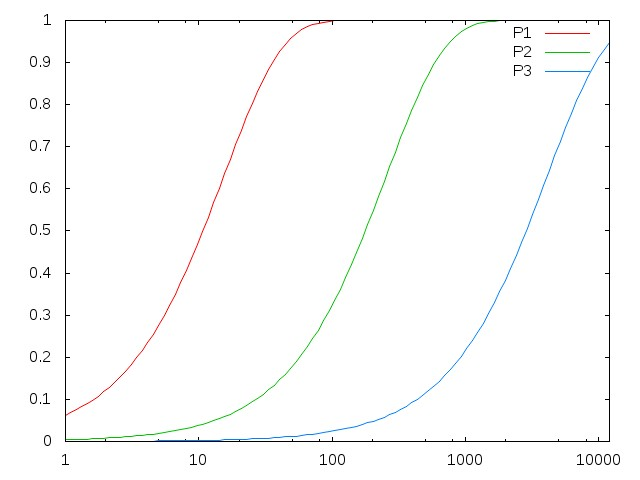
\includegraphics[width=0.8\textwidth]{plot.jpg}
  \end{figure}
  \begin{scriptsize}
    To get the right hash with a probability of 95\%:
    \begin{itemize}
      \item 1 character $\Rightarrow$ 46 attempts $\Rightarrow\ < 1$ms
      \item 2 character $\Rightarrow$ 765 attempts $\Rightarrow\ \sim 6$ms
      \item 3 character $\Rightarrow$ 12269 attempts $\Rightarrow\ \sim100$ms
    \end{itemize}
  \end{scriptsize}
\end{frame}

\subsection{Author/Committer}

\begin{frame}
  \frametitle{\insertsubsectionhead}
  \begin{small}
    commit 231tree cc7e48bd538188f75551fac0972840a7f6c2401f\\
    parent 31463d4a762389f9b3d8fe872971e27c14dec645\\
    author \textbf{Charles De Latourette} \textless cl@gmail.com\textgreater 1412964284 -0400\\
    committer \textbf{Fran\c{c}ois \'Edouard} \textless fe@gmail.com\textgreater 1412964284 -0400\\
    commit message
  \end{small}
\end{frame}

\begin{frame}
  \frametitle{\insertsubsectionhead}
  \textbf{How many possible values on a single commit?}\\
  Number of ordered combinations between the contributors:\\
  $C(n) = \frac{n!}{(n-2)!}$\\
  
  \medskip
  \medskip
  \medskip
  
  12 contributors $\Rightarrow$ 132 possible values $\Rightarrow\ \sim$ 7 bits per commit
\end{frame}


\subsection{Format of the source code}

\begin{frame}
  \frametitle{\insertsubsectionhead}
  \begin{itemize}
    \item Alternate between indentations with spaces and with tabulations
    \item []
    \item Alternate between CR+LF and LF for the newlines
  \end{itemize}
\end{frame}

\begin{frame}
  \frametitle{\insertsubsectionhead}
  \begin{itemize}
    \item Source code management softwares preserve the format
    \item []
    \item Indentations and new lines characters are "invisible"
    \item []
    \item Many projects without coding conventions
  \end{itemize}
\end{frame}

\begin{frame}
  \frametitle{\insertsubsectionhead}
  \textbf{How much can we hide in a line of code?}\\
  4 possibilities for indented lines $\Rightarrow$ 2 bits per line
\end{frame}

\subsection{Behavior-based covert channels}

\begin{frame}
  \frametitle{\insertsubsectionhead}
  \begin{itemize}
  \item Order in which the files are committed
   \end{itemize}
\end{frame}

\begin{frame}
  \frametitle{\insertsubsectionhead}
\begin{itemize}
  \item Really difficult to detect without an understanding of the project
  \item []
  \item Faster than similar behavior-based covert channels in web browser for example
  \item []  
  \item Can make and push all commits at once to transmit more data 
\end{itemize}
\end{frame}

\section{Conclusion}

\begin{frame}
\frametitle{\insertsectionhead}
\begin{itemize}
	\item Entropy measurements to improve the stealthiness
    \item []
    \item Complete study of behaviour-based covert channels
    \item []
	\item Need to look to other tools, like SVN or Mercurial
\end{itemize}
\end{frame}

\begin{frame}
  \frametitle{\insertsectionhead}
  Questions or comments?
\end{frame}


\end{document}
